\documentclass{article}
\usepackage{amsmath,amssymb}
\usepackage{graphicx}
\usepackage{enumerate}
\usepackage{hyperref}
\usepackage{subcaption}
\usepackage{caption}
\usepackage{xcolor}
\usepackage{float}
\usepackage{xcolor}
\hypersetup{
    colorlinks,
    linkcolor={red!50!black},
    citecolor={blue!50!black},
    urlcolor={blue!80!black}
}

\pagestyle{empty} \addtolength{\textwidth}{1.0in}
\addtolength{\textheight}{0.5in}
\addtolength{\oddsidemargin}{-0.5in}
\addtolength{\evensidemargin}{-0.5in}
\newcommand{\ruleskip}{\bigskip\hrule\bigskip}
\newcommand{\nodify}[1]{{\sc #1}}
\newcommand{\points}[1]{{\textbf{[#1 points]}}}
\newcommand{\subquestionpoints}[1]{{[#1 points]}}
\newenvironment{answer}{{\bf Answer:} \sf }{}%

\newcommand{\bitem}{\begin{list}{$\bullet$}%
{\setlength{\itemsep}{0pt}\setlength{\topsep}{0pt}%
\setlength{\rightmargin}{0pt}}}
\newcommand{\eitem}{\end{list}}

\setlength{\parindent}{0pt} \setlength{\parskip}{0.5ex}
\setlength{\unitlength}{1cm}

\newcommand{\pa}[1]{[[PA: #1]]}

\renewcommand{\Re}{{\mathbb R}}
\newcommand{\E}{{\rm E}}
\begin{document}

\pagestyle{myheadings} \markboth{}{COMP447-547 Deep Unsupervised Learning, Homework 1, Spring 2022}

{\huge
\noindent Homework 1: Autoregressive Models}
\ruleskip

{\bf Deliverable}: This PDF write-up by {\bf Wednesday March 16th, 23:59pm}.  Your PDF should be generated by simply replacing the placeholder images of this LaTeX document with the appropriate solution images that will be generated automatically when solving each question. The solution images are automatically generated and saved using the accompanying IPython notebook. Download your results from Google Colab and replace the images in the figures/ folder with your result images. Write your name and ID in the necessary parts below, confirming the Honor Pledge. Then, you will run the .tex file to generate your PDF file. Your PDF is to be submitted into Blackboard along with your notebook, please follow the instructions given in the GitHub page. This PDF already contains a few solution images.  These images will allow you to check your own solution to ensure correctness.

{\bf Honor Pledge}: ``I affirm that I have not given or received any unauthorized help on this assignment, and that this work is my own."

{\bf Name}: YOUR NAME HERE

{\bf ID}: YOUR ID HERE

\vspace{.1in}

{\bf Note}: \textit{This assignment is adapted from UC Berkeley \href{https://sites.google.com/view/berkeley-cs294-158-sp20/home}{CS294-158-SP20}}
\vspace{.2in}

%--------------------------------------------------------------------------------
%--------------------------------------------------------------------------------
%--------------------------------------------------------------------------------
\noindent {\bf Question 1: 1D Data}
%--------------------------------------------------------------------------------
%--------------------------------------------------------------------------------
%--------------------------------------------------------------------------------

\begin{enumerate}[(a)]

\item {\bf [5pt] Fitting a Histogram} \\\\
Final test loss for dataset 1: \textcolor{red}{FILL IN HERE}nats / dim
\begin{figure}[H]
    \centering
    \begin{subfigure}{0.45\textwidth}
        \centering
        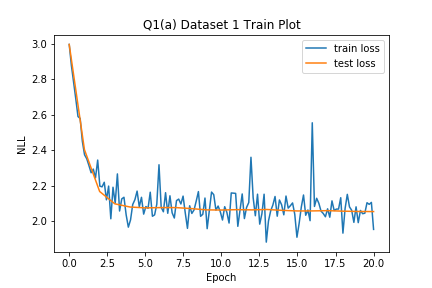
\includegraphics[width=\textwidth]{figures/q1_a_dset1_train_plot.png}
        \caption{Dataset 1: Training curve}
    \end{subfigure}
    \hspace{0.2in}
    \begin{subfigure}{0.45\textwidth}
        \centering
        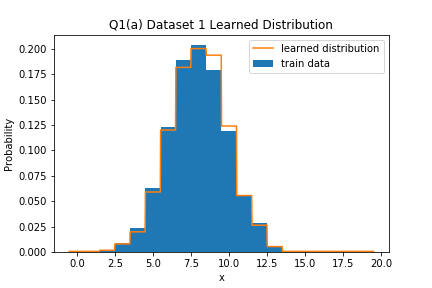
\includegraphics[width=\textwidth]{figures/q1_a_dset1_learned_dist.png}
        \caption{Dataset 1: Learned distribution}
    \end{subfigure}
\end{figure}

\newpage

Final test loss for dataset 2: \textcolor{red}{FILL IN HERE} nats / dim
\begin{figure}[H]
    \centering
    \begin{subfigure}{0.45\textwidth}
        \centering
        
\includegraphics[width=\textwidth]{figures/q1_a_dset2_train_plot.png}
        \caption{Dataset 2: Training curve}
    \end{subfigure}
    \hspace{0.2in}
    \begin{subfigure}{0.45\textwidth}
        \centering
        
\includegraphics[width=\textwidth]{figures/q1_a_dset2_learned_dist.png}
        \caption{Dataset 2: Learned distribution}
    \end{subfigure}
\end{figure}

\newpage

\item {\bf [5pt] Fitting Discretized Mixture of Logistics} \\\\
Final test loss for dataset 1: \textcolor{red}{FILL IN HERE} nats / dim
\begin{figure}[H]
    \centering
    \begin{subfigure}{0.45\textwidth}
        \centering
        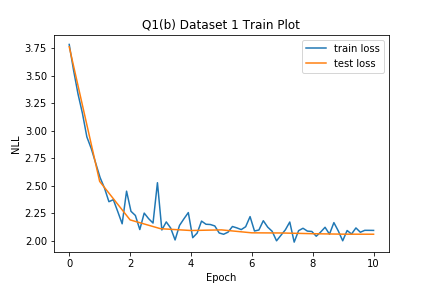
\includegraphics[width=\textwidth]{figures/q1_b_dset1_train_plot.png}
        \caption{Dataset 1: Training curve}
    \end{subfigure}
    \hspace{0.2in}
    \begin{subfigure}{0.45\textwidth}
        \centering
        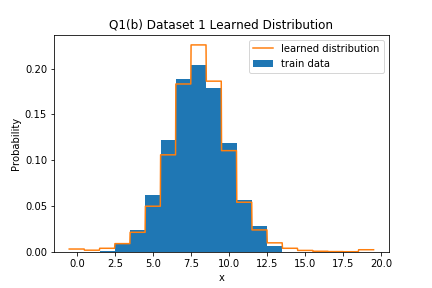
\includegraphics[width=\textwidth]{figures/q1_b_dset1_learned_dist.png}
        \caption{Dataset 1: Learned distribution}
    \end{subfigure}
\end{figure}
Final test loss for dataset 2: \textcolor{red}{FILL IN HERE}  nats / dim
\begin{figure}[H]
    \centering
    \begin{subfigure}{0.45\textwidth}
        \centering
        
\includegraphics[width=\textwidth]{figures/q1_b_dset2_train_plot.png}
        \caption{Dataset 2: Training curve}
    \end{subfigure}
    \hspace{0.2in}
    \begin{subfigure}{0.45\textwidth}
        \centering
        
\includegraphics[width=\textwidth]{figures/q1_b_dset2_learned_dist.png}
        \caption{Dataset 2: Learned distribution}
    \end{subfigure}
\end{figure}
\end{enumerate}


%--------------------------------------------------------------------------------
%--------------------------------------------------------------------------------
%--------------------------------------------------------------------------------
\newpage
\noindent {\bf Question 2: PixelCNNs}
%--------------------------------------------------------------------------------
%--------------------------------------------------------------------------------
%--------------------------------------------------------------------------------

\begin{enumerate}[(a)]
\item {\bf [10pt] PixelCNN on MNIST} \\\\
Final test loss: \textcolor{red}{FILL IN HERE}   nats / dim
\begin{figure}[H]
    \centering
    \begin{subfigure}{0.45\textwidth}
        \centering
        
\includegraphics[width=\textwidth]{figures/q2_a_train_plot.png}
        \caption{Dataset 1: Training curve}
    \end{subfigure}
    \hspace{0.2in}
    \begin{subfigure}{0.45\textwidth}
        \centering
        
\includegraphics[width=\textwidth]{figures/q2_a_samples.png}
        \caption{Dataset 1: Samples}
    \end{subfigure}
\end{figure}

\newpage

\item {\bf [15pt] PixelCNN+ on MNIST} \\\\
Final test loss: \textcolor{red}{FILL IN HERE}   nats / dim
\begin{figure}[H]
    \centering
    \begin{subfigure}{0.45\textwidth}
        \centering
        
\includegraphics[width=\textwidth]{figures/q2_b_train_plot.png}
        \caption{Dataset 1: Training curve}
    \end{subfigure}
    \hspace{0.2in}
    \begin{subfigure}{0.45\textwidth}
        \centering
        
\includegraphics[width=\textwidth]{figures/q2_b_samples.png}
        \caption{Dataset 1: Samples}
    \end{subfigure}
\end{figure}

\newpage

\item {\bf [15pt] GatedPixelCNN on MNIST} \\\\
Final test loss: \textcolor{red}{FILL IN HERE}  nats / dim
\begin{figure}[H]
    \centering
    \begin{subfigure}{0.45\textwidth}
        \centering
        
\includegraphics[width=\textwidth]{figures/q2_c_train_plot.png}
        \caption{Dataset 1: Training curve}
    \end{subfigure}
    \hspace{0.2in}
    \begin{subfigure}{0.45\textwidth}
        \centering
        
\includegraphics[width=\textwidth]{figures/q2_c_samples.png}
        \caption{Dataset 1: Samples}
    \end{subfigure}
\end{figure}
\end{enumerate}

\end{document}
